\documentclass[a4paper,10pt]{article}
\usepackage[utf8]{inputenc}
\usepackage{graphicx}

% Title Page
\title{Very brief progress report on NLTE inversions}
\author{Ivan Mili\'{c}}


\begin{document}
\maketitle

\section{Status from the summer (last meeting)}
At the moment of our last meeting we had quite reliable method for computing level responses to changes in temperature, density and microturbulent velocity. Method has been tested on a prototype 2-level line with atomic parameters (abundance, energy levels, Einstein coefficients) corresponding to H$\alpha$ line (so, very optically thick line which is in, so to say, extreme NLTE conditions). For the publication of the results we have also tested the method on CaII 5-level atom. For both examples we had excellent agreement between the analytical and finite-difference responses. 

We also implemented 'propagation' of these responses in order to compute responses of emergent scalar intensity. As expected, they also showed excellent agreement with the finite-difference intensity response functions. 

The results and method are in the manuscript which has recently been accepted to A\&A (also attached to the e-mail). 

\section{Progress during last several months}

In the meantime, we extended the code so it can now compute responses of polarized opacity and emissivity to all the relevant quantities (temperature, density, microturbulent and systematic velocity, magnetic field vector), and propagate them using polarized solver to compute polarized spectrum and its responses. This can be done both for $h$ and $\tau_{500}$ as spatial grid. The first one is useful for forward calculations and approximate diagnostics (i.e. using semi-empirical model atmospheres), while the latter is necessary for inversion scheme.

Since we already had a scalar inversion scheme set-up, it took minimal work to extend it to more atmospheric parameters and full Stokes case. The inversion works, and retrieves atmospheric parameters back to an original model down to numerical accuracy. However, (Fig.\,1) it does not converge as fast as one based on numerical derivatives. Example is for a simple atmosphere with four nodes in temperature and one node for each of other parameters. 
\begin{figure}
 \includegraphics[width = 10cm]{convergence_comparison.eps}
 \caption{Comparison of noise-free inversion based on analytical and finite-difference response functions.}
\end{figure}
The reason for this is probably a coding error which induces small, but noticeable discrepancy to perturbations in some, less important, nodes, which in turn slows down the convergence. As scalar inversions are working perfectly, we expect to hunt down the error soon. 

We also implemented an approximate computation for scattering polarization and its responses. It only work for simple atomic models (2-level atom, unpolarized lower level). Response functions to scattering polarization have very interesting shape and seem to span greater range of heights that intensity response functions. Example is given in Fig.\,2. 
\begin{figure}
 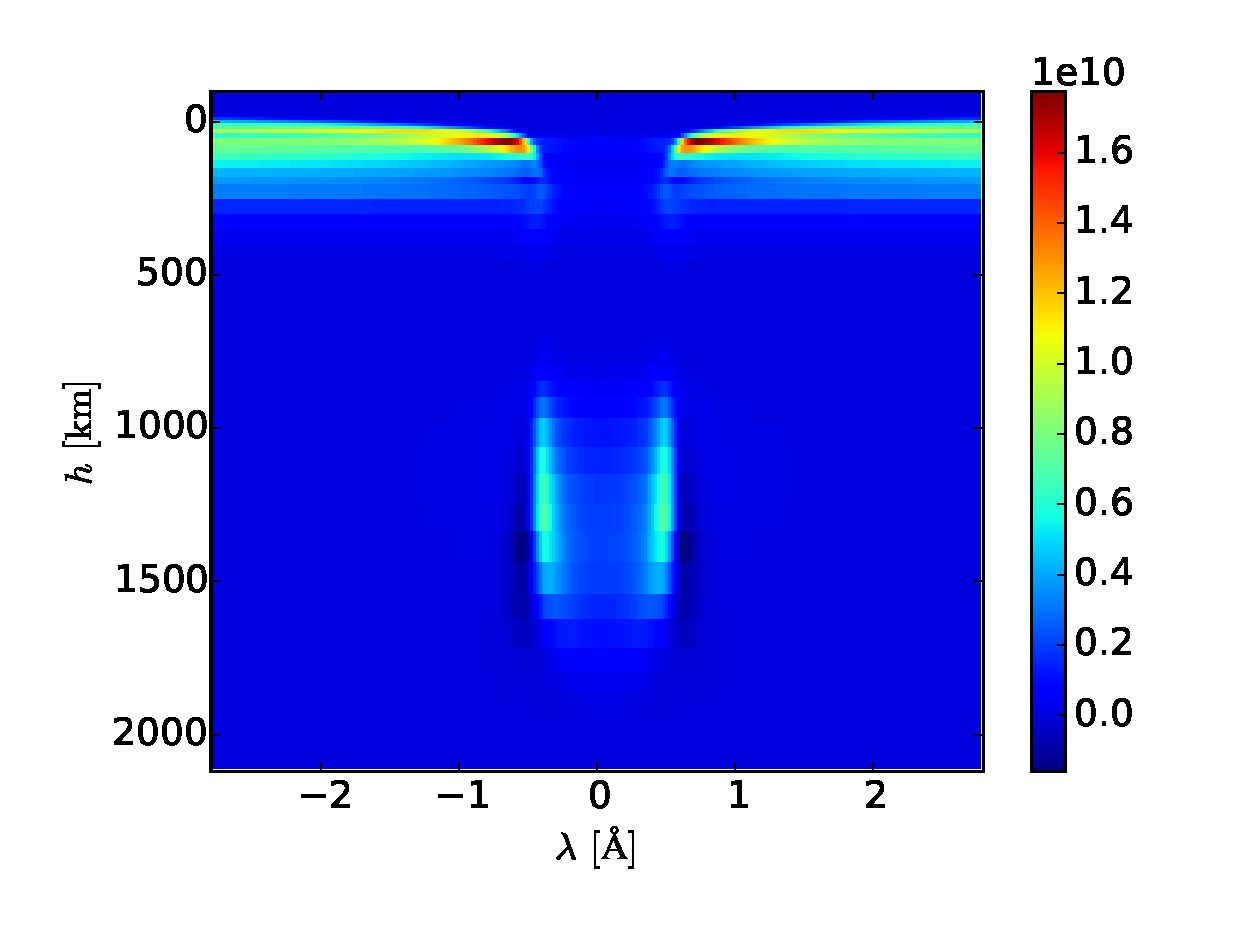
\includegraphics[width=5cm]{I.eps}
 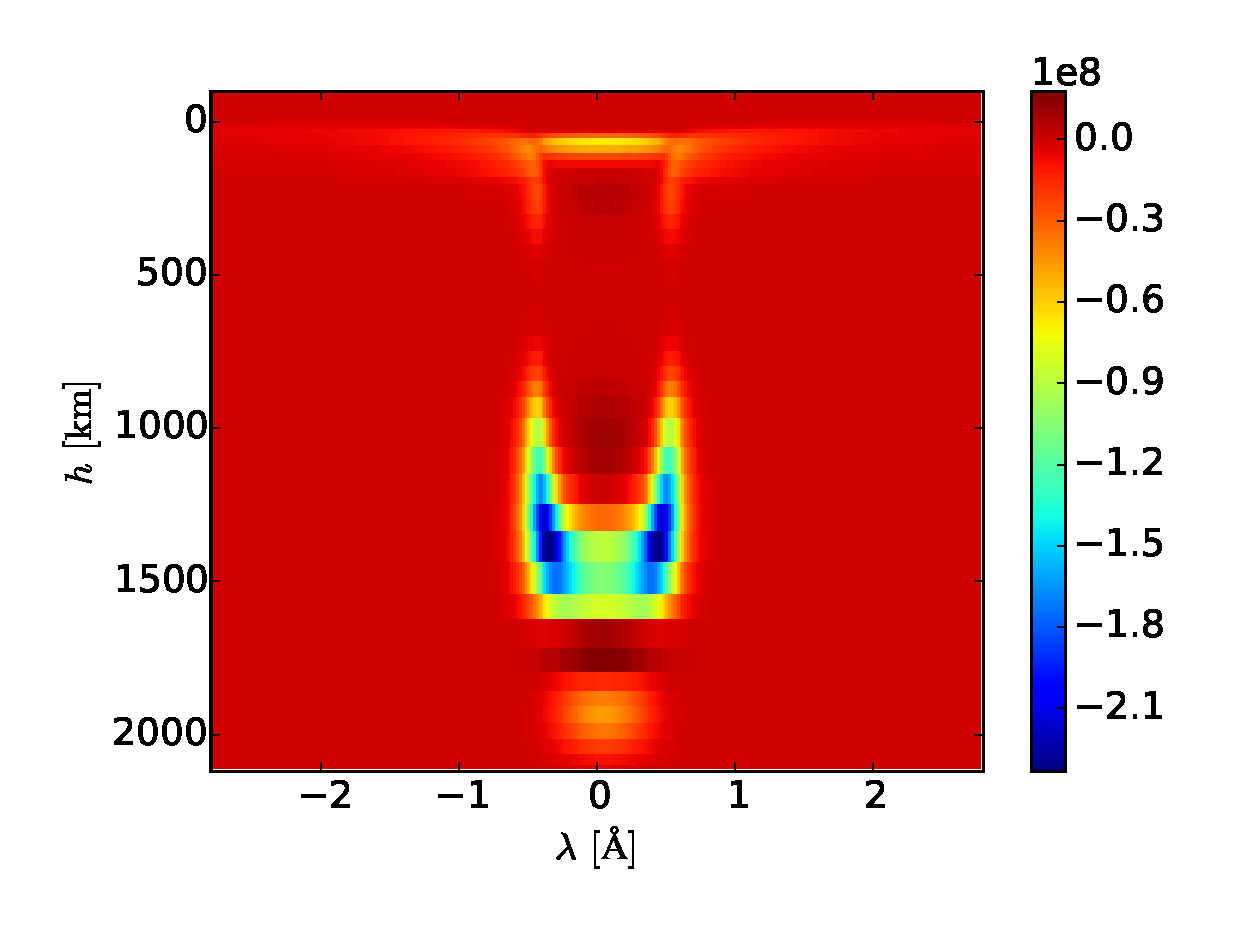
\includegraphics[width=5cm]{Q.eps}
 \caption{Intensity (left) and scattering polarization (right) response functions to temperature for a prototype 2-level NLTE line in FALC model atmosphere at $\mu=0.5$.}
\end{figure}
Response functions to scattering polarization have not been used so far, neither has any kind of Hanle inversion been based on them. This could potentially prove to be a very useful diagnostics tool should be get to work with spatially-resolved observations of scattering polarization.

\section{Further steps}

In order to make the code usable with the observations, following steps need to be undertaken: 
\begin{itemize} 
 \item Find the source of discrepancy in convergence rate and show that analytical responses work as well as numerical ones for Zeeman NLTE inversion. 
 \item Extensively test the code for the lines we are interested in, for various atmospheric and atomic models (we need simple but yet realistic atomic models). 
 \item Optimize the code and make it parallel (as it will be used in pixel-by-pixel mode, observed region can be simply split between the processes). 
\end{itemize}

Personally, I would like to investigate further the responses of scattering polarization and , in collaboration with other SLAM members, perhaps propose some simple diagnostics, which might be interesting for next SUNRISE flight. 

\newpage

\section{Na response functions}

Due to the fact we have Na D1 observations from SST from last summer, Michiel and me wanted to explore possibility or inverting SP observations in these lines. First step was to see if our code can reproduce the shape of the line properly and to compute response function. All the examples below are for FALC model atmosphere, and magnetic field  with magnitude 1000\,G, inclination 30 degrees and azimuth 30 degrees. They agree qualitatively with what Uitenbroek (2006) computes (although he uses MHD snapshots).

\begin{figure}
 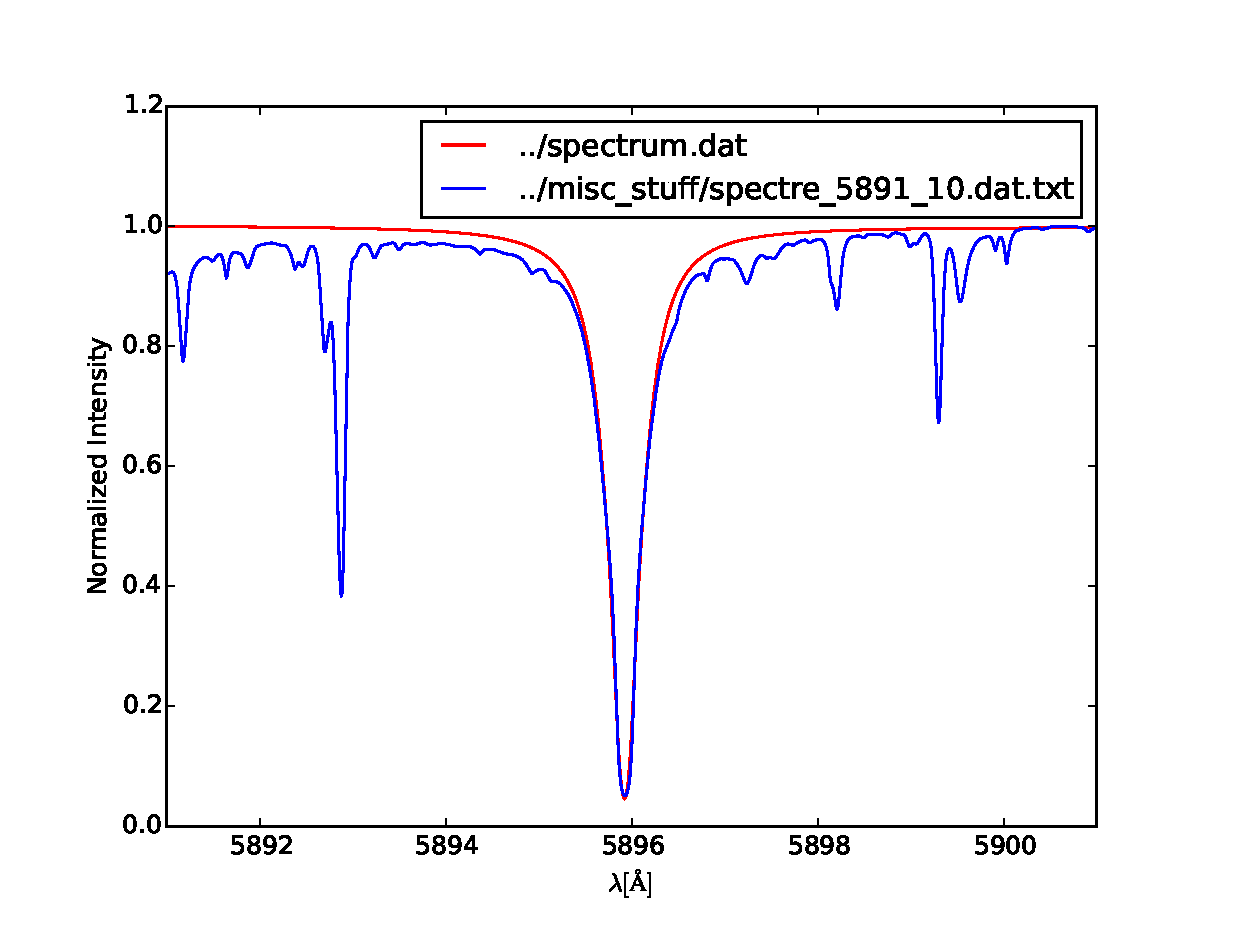
\includegraphics[width=8cm]{Na_test.eps}
 \caption{Comparison between calculated spectra, including 2km/s macroturbulence broadening and FTS atlas.}
\end{figure}
\begin{figure}
 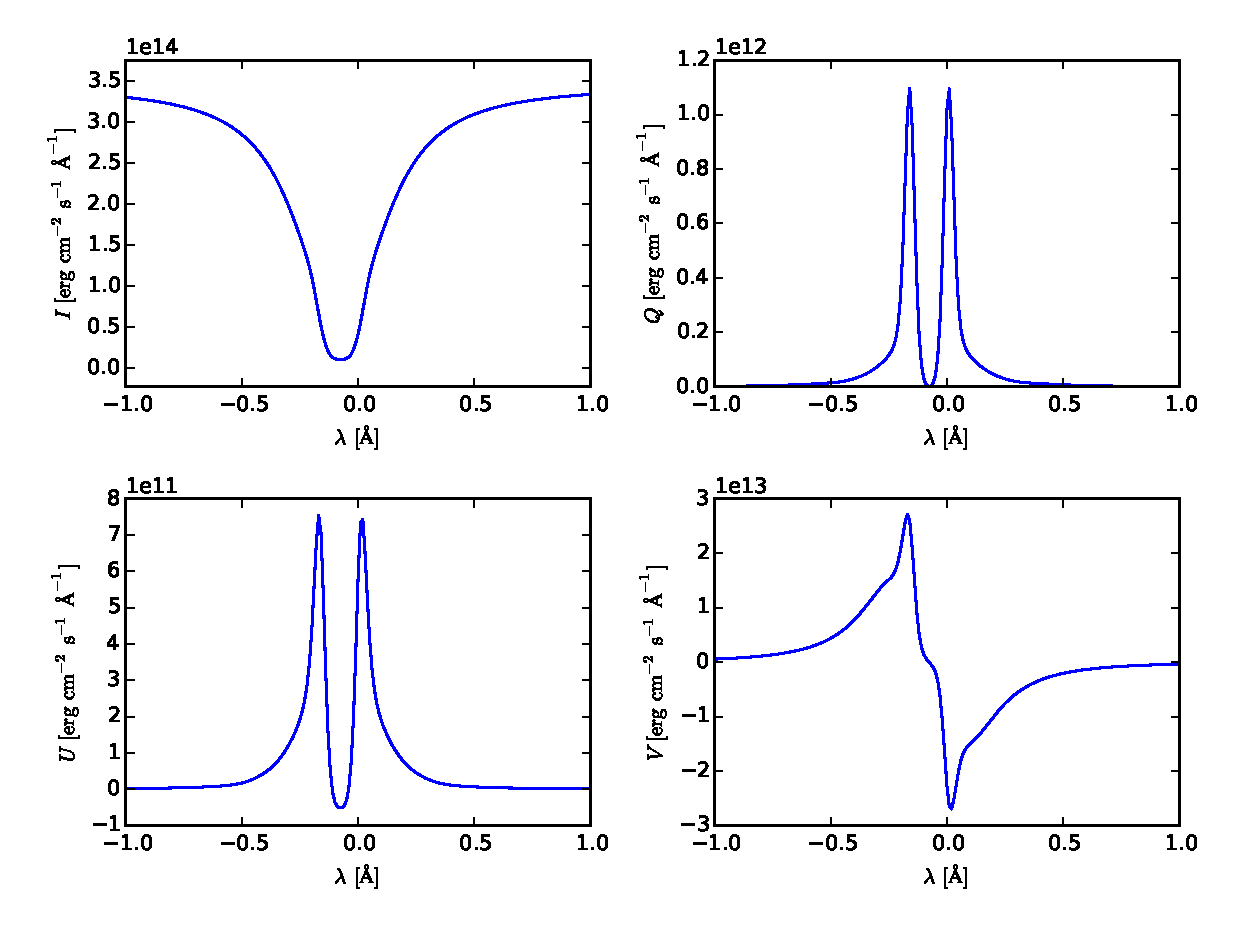
\includegraphics[width=8cm]{Na_stokes_stokes_spectrum.eps}
 \caption{Stokes spectra of Na D1 line assuming constant magnetic field with magnitude 1000\,G, inclination 30 degrees and azimuth 30 degrees.}
\end{figure}
\begin{figure}
 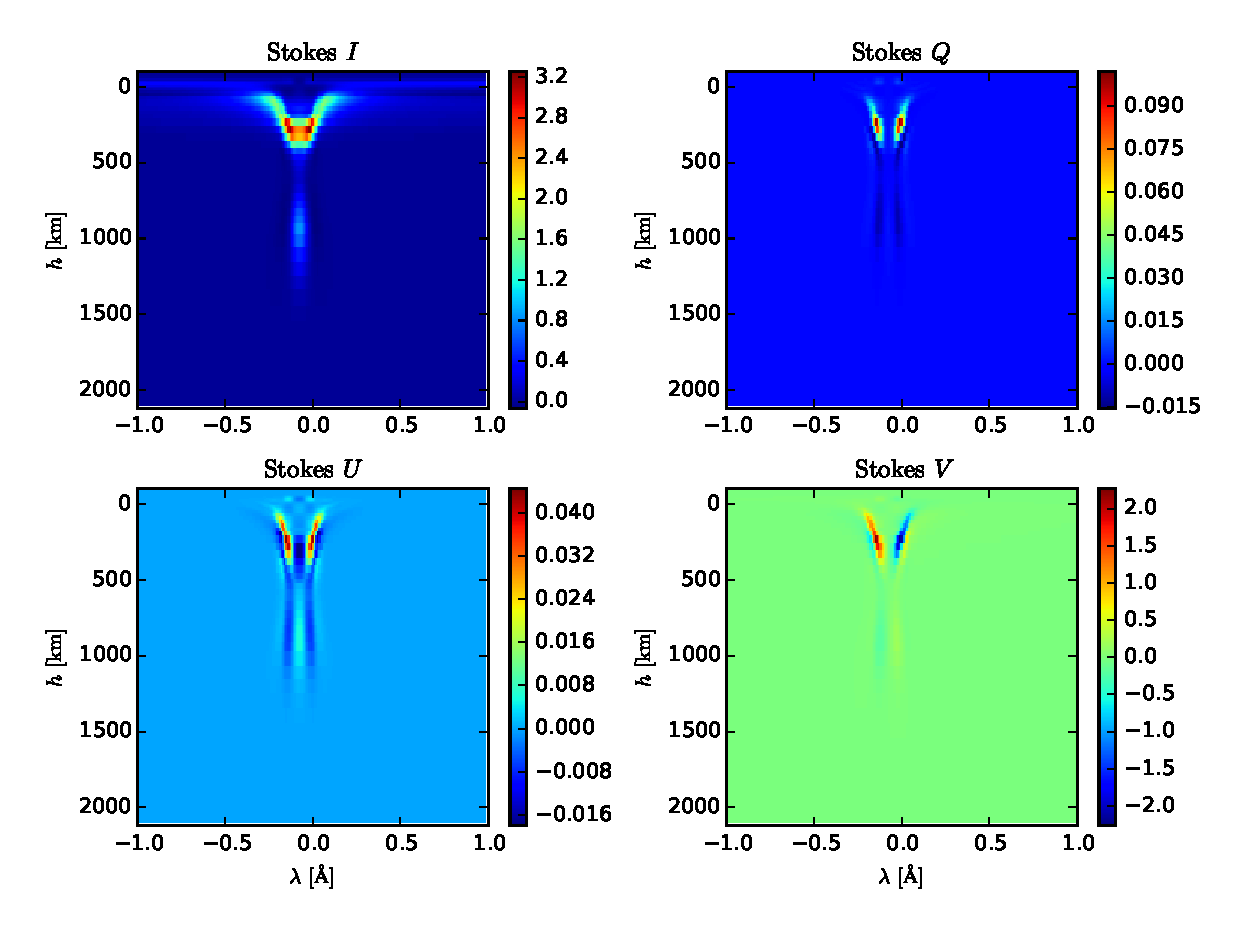
\includegraphics[width=\textwidth]{Na_stokes_analytical_responses_intensity_temperature.eps}
 \caption{Stokes response function to temperature for Na D1.}
\end{figure}
\begin{figure}
 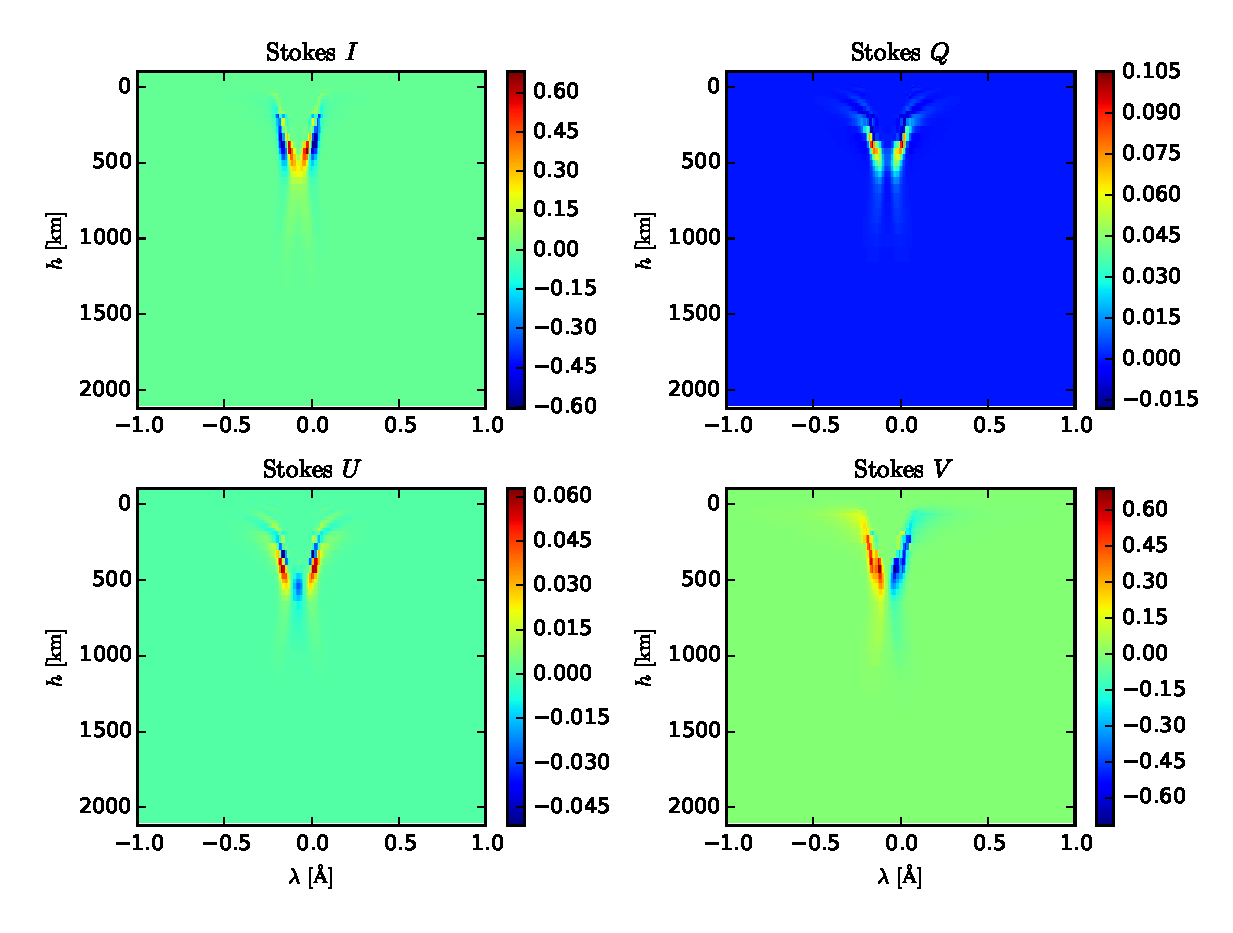
\includegraphics[width=\textwidth]{Na_stokes_analytical_responses_intensity_B.eps}
 \caption{Stokes response function to magnetic field for Na D1.}
 \end{figure}
 
We are still not completely sure what causes difference in convergence between inversions based on analytical and numerical schemes. I found some ``errors'', but there is still some discrepancy. All tests so far go like this: 
\begin{enumerate}
 \item Set-up ad-hoc atmosphere based on nodes. Compute spectrum.
 \item Invert spectrum with the aim of getting back original nodes down to numerical precision (this should happen relatively fast, in <20 iterations for sure). 
\end{enumerate}
First thing that is to be noted here, and I think it is the consequence of problem being in NLTE is that, depending on the starting guess, you mind end up with unreasonable solution and inversion scheme might explode, even when using numerical derivatives. With decent initial guess tho, both responses work very good, but analytical one is lagging. Here is the demonstration for varying number of Temperature nodes (other quantities have one node):

\begin{figure}
 \includegraphics[width=8cm]{convergence2.eps}
 \includegraphics[width=8cm]{convergence3.eps}
 \includegraphics[width=8cm]{convergence4.eps}
 \includegraphics[width=8cm]{convergence5.eps}
\end{figure}



\end{document}          
